% Copyright 2024 Kieran W Harvie. All rights reserved.

\section{Bézier Triangles}
Let $\mathbf{\lambda}$ be an $n$ dimensional vector and let $S = \{0\leq k\leq n-1\}^n$
\[
	f(\mathbf{\lambda}) =\sum_{s\in S}\mathbf{P}_s\prod_{k=0}^{n-1}\lambda_k\\
\]
Where for all permulations $\sigma$ we have:
\[
	\mathbf{P}_{\sigma(s)} = \mathbf{P}_s
\]
\[\begin{aligned}
	f(\lambda_0,\lambda_1,\lambda_2) =& \lambda_0^3\mathbf{P}_{0,0,0}+\lambda_1^3\mathbf{P}_{1,1,1}+\lambda_2^3\mathbf{P}_{2,2,2}\\
	&+3\lambda_0^2\lambda_1\mathbf{P}_{0,0,1}+3\lambda_0^2\lambda_2\mathbf{P}_{0,0,2}\\
	&+3\lambda_1^2\lambda_0\mathbf{P}_{0,1,1}+3\lambda_1^2\lambda_2\mathbf{P}_{1,1,2}\\
	&+3\lambda_2^2\lambda_0\mathbf{P}_{0,2,2}+3\lambda_2^2\lambda_1\mathbf{P}_{1,2,2}\\
	&+6\lambda_0\lambda_1\lambda_2\mathbf{P}_{0,1,2}\\
\end{aligned}\]
Given $10$ control points $\{\mathbf{P}_{i,j,k}\mid i,j,k\geq 0 \text{ and }i+j+k=3\}$ the Cubic Bézier triangle is the region:
\[\begin{aligned}
&\lambda_0^3\mathbf{P}_{3,0,0}+\lambda_1^3\mathbf{P}_{0,3,0}+\lambda_2^3\mathbf{P}_{0,0,3}\\
&+3\lambda_0^2\lambda_1\mathbf{P}_{2,1,0}+3\lambda_0^2\lambda_2\mathbf{P}_{2,0,1}\\
&+3\lambda_1^2\lambda_0\mathbf{P}_{1,2,0}+3\lambda_1^2\lambda_2\mathbf{P}_{0,2,1}\\
&+3\lambda_2^2\lambda_0\mathbf{P}_{1,0,2}+3\lambda_2^2\lambda_1\mathbf{P}_{0,1,2}\\
&+6\lambda_0\lambda_1\lambda_2\mathbf{P}_{1,1,1}\\
\end{aligned}\]
Such that:
\[\lambda_0+\lambda_1+\lambda_2 = 1,\text{ and } \lambda_0,\lambda_1,\lambda_2\geq0\]
This expression is quite verbose but is visually quite intuitive:
\begin{center}
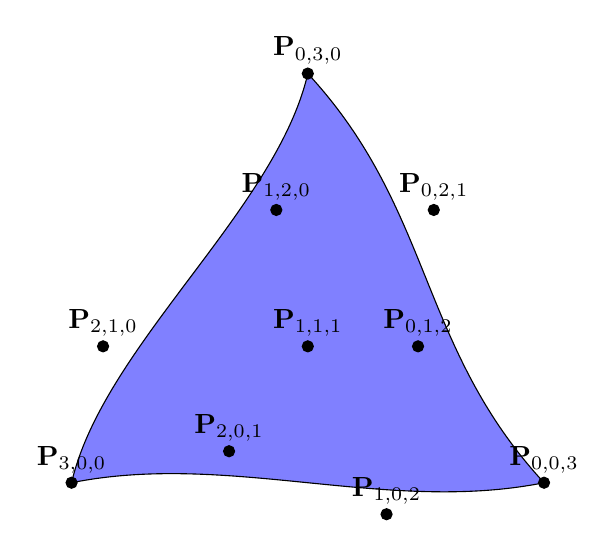
\begin{tikzpicture}[every node/.style={black}]
%	\coordinate (    ) at (Y+Z*2    , Y*1.7320508075    );
\coordinate (p300) at (0+0*2    , 0*1.7320508075    );
\coordinate (p210) at (1+0*2-0.6, 1*1.7320508075    );
\coordinate (p201) at (0+1*2    , 0*1.7320508075+0.4);
\coordinate (p120) at (2+0*2+0.6, 2*1.7320508075    );
\coordinate (p111) at (1+1*2    , 1*1.7320508075    );
\coordinate (p102) at (0+2*2    , 0*1.7320508075-0.4);
\coordinate (p030) at (3+0*2    , 3*1.7320508075    );
\coordinate (p021) at (2+1*2+0.6, 2*1.7320508075    );
\coordinate (p012) at (1+2*2-0.6, 1*1.7320508075    );
\coordinate (p003) at (0+3*2    , 0*1.7320508075    );
\coordinate (p300) at (0+0*2    , 0*1.7320508075    );

\filldraw[fill=blue!50] (p300) .. controls (p210) and (p120) ..  (p030) .. controls (p021) and (p012) .. (p003) .. controls (p102) and (p201) .. (p300);

\filldraw (p300) node[above]{$\mathbf{P}_{3,0,0}$} circle(2pt);
\filldraw (p210) node[above]{$\mathbf{P}_{2,1,0}$} circle(2pt);
\filldraw (p201) node[above]{$\mathbf{P}_{2,0,1}$} circle(2pt);
\filldraw (p120) node[above]{$\mathbf{P}_{1,2,0}$} circle(2pt);
\filldraw (p111) node[above]{$\mathbf{P}_{1,1,1}$} circle(2pt);
\filldraw (p102) node[above]{$\mathbf{P}_{1,0,2}$} circle(2pt);
\filldraw (p030) node[above]{$\mathbf{P}_{0,3,0}$} circle(2pt);
\filldraw (p021) node[above]{$\mathbf{P}_{0,2,1}$} circle(2pt);
\filldraw (p012) node[above]{$\mathbf{P}_{0,1,2}$} circle(2pt);
\filldraw (p003) node[above]{$\mathbf{P}_{0,0,3}$} circle(2pt);

\end{tikzpicture}

An example Cubic Bézier Triangle with control points shown.
\end{center}
